\documentclass[10pt,letterpaper]{article}
\usepackage[utf8]{inputenc}
\usepackage[english]{babel}
\usepackage{amsmath}
\usepackage{amsfonts}
\usepackage{amssymb}
\usepackage{graphicx}
\graphicspath{{../Figures/}}
\usepackage{hyperref}
\usepackage{apacite}
\usepackage{booktabs}
\usepackage{subcaption}
\usepackage[left=2cm,right=2cm,top=2cm,bottom=2cm]{geometry}
\setlength{\parskip}{\baselineskip}%
\setlength{\parindent}{0pt}%

\usepackage[compact]{titlesec}
\titlespacing{\section}{0pt}{*0}{*0}
%\titlespacing{\subsection}{0pt}{*0}{*0}
%\titlespacing{\subsubsection}{0pt}{*0}{*0}

\author{Silas Mann \and Jonas Peeters}
\title{DS-GA 1017 Project: Fairness in Sepsis Detection}
\date{\today}
\begin{document}
\maketitle
\vspace*{-1cm}

% \pagenumbering{gobble}

% DRAFT BACKGROUND AND INPUT AND OUTPUT SECTIONS

\section*{Background}

% 1. Background: general information about your chosen ADS
%	a. What is the purpose of this ADS? What are its stated goals?
%	b. If the ADS has multiple goals, explain any trade-offs that these goals may introduce.

\par Sepsis is a life-threatening dysfunctional immune response to infection in which the body attacks its own tissues and organs, often leading to organ failure and death \cite{Singer2016}. It is a critically important world-wide public health issue; with a mortality rate of about 16\%, the estimated number of world-wide cases is as high as 31.5 million \cite{Fleischmann2016}, and in the United States alone over 1.7 million develop sepsis annually\footnote{\href{https://www.cdc.gov/sepsis/clinicaltools/index.html?CDC_AA_refVal=https\%3A\%2F\%2Fwww.cdc.gov\%2Fsepsis\%2Fdatareports\%2Findex.html}{https://www.cdc.gov/sepsis/clinicaltools.html}}. Better outcomes and lower mortality rates have been connected to early treatment, including the administration of early antibiotics and fluids \cite{Rhee2018}. However, early identification of sepsis remains a challenge. Much work has been done in an effort to develop early identification strategies in the clinical setting \cite{Kim2019}, and in recent years, these efforts have turned toward the use of automated decision systems based on machine learning to predict sepsis \cite{Fleuren2020} and identify patients who may benefit from treatment programs such as early-goal directed therapy (EGDT) or SSC bundles \cite{Kim2019}. In an effort to advance these efforts, PhysioNet, a repository for freely-available medical research data, launched a 2019 challenge entitled “Early Prediction of Sepsis from Clinical Data” \cite{Reyna2019}.

\par The use of machine learning models to assess the state of patients' health and determine whether to initiate preemptive procedures is relatively new. In the case of sepsis, if such a model is able to correctly predict risk, it has the opportunity to prevent life-threatening illness, whereas if the model fails to predict risk, the consequences can be grave. Constrastingly, if the model incorrectly predicts sepsis, vital resources may be allocated to a patient that would have better allocated to another patient. Frequent incorrect predictions can also result in alert fatigue; doctors may choose to ignore the predictions if they tend to be incorrect.  Given the gravity of the consequences, it is paramount that such models do not further perpetuate differences in medical treatment for historically unprivileged groups. For example, \citeauthor{Greenwood2018} found that female patients are less likely than their male counterparts to survive traumatic health episodes such as heart attacks. A model that informs doctors on the risk of sepsis could either reinforce existing biases in medical care or potentially lessen them by offering a more impartial assessment than may be provided by the largely male medical staff found in ICUs \cite{Chadwick2020}.

\par In 2019, \citeauthor{Sindwani2019} published an article in Towards Data Science titled “Early Detection of Sepsis Using Physiological Data". In the article, Sindwani outlines the problem above. The paper includes exploratory data analysis, feature selection/engineering, and model training and evaluation. Sindwani also provides a link to a fully functioning GitHub \cite{Karan2019}. We chose the best model provided by the author to analyze for fairness. 

\par First, we determine if there are any existing biases in the dataset that may lead to less favorable outcomes for marginalized groups. We explore underlying evidence of disparate impact between the privileged and unprivileged groups for the 'gender' variable. Next, consider the preprocessing steps taken by the author, and identify any steps that introduce additional bias. We then explore the results of the model and analyze whether the model introduces or perpetuates any bias between groups, considering disparate impact, mean difference, and false positive rates. Most medical data are provided at the level of the individual patient, and several precautions are taken to ensure the privacy of the individuals included in the data set. Therefore we discuss the possible pitfalls of the privacy measures implemented in releasing this dataset for the competition.

\section*{Input and output}

% 2. Input and output
%	a. Describe the data used by this ADS. How was this data collected or selected?
%	b. For each input feature, describe its datatype, give information on missing values and on the value distribution. Show pairwise correlations between features if appropriate. Run any other reasonable profiling of the input that you find interesting and appropriate.
%	c. What is the output of the system (e.g., is it a class label, a score, a probability, or some other type of output), and how do we interpret it?

\par The training data, which were provided in the PhysioNet website to anyone interested in participating, were sourced from 40,000 ICU patients from Beth Israel Deaconess Medical Center and Emory University Hospital. While the test data do not appear to have ever been released, the training data are still available for download in the PhysioNet archive \cite{Goldberger2000}. The deidentified data for each patient are contained within a single pipe-delimited file, and include demographics, vitals, and laboratory values, and binary sepsis onset defined on relevant events (time of initial clinical suspicion, time of deterioration in organ failure assessment, and time of sepsis onset).

\par Time of initial clinical suspicion of infection was defined as either the time IV antibiotics or blood cultures, whichever came first. To be considered, antibiotics must have been ordered within 3 days after blood cultures, and blood cultures must have been ordered within 1 day of antibiotics, with at least 3 days of consecutive antibiotics treatment. Organ damage was defined as 2-point deterioration in SOFA score within 1 day. Time of sepsis was defined as either time of clinical suspicion of infection or end time of organ failure assessment, whichever came first, as long as organ damage occurred 2 days before or 1 day after suspicion of infection. A patient was labeled as having sepsis if time is greater than or equal to time of sepsis minus 6 hours.

\par The original data provided by the PhysioNet challenge are temporal: a single row in the data set is not an individual, but a rather a time point. The author of the prediction tool chose to ignore the time component, and treat each record as independent and identically distributed. The author argues that this approach could be used to predict sepsis at each hour for a given patient without taking into account past data.

% ***elaborate on how this is not a good assumption and what issues it may cause

\par The sepsis binary indicator is our label of interest. A value of zero represents the patient without sepsis within 6 hours, and a value of one represents the patient having sepsis within 6 hours. We can see in Figure \ref{fig:label_dist} that the data are unbalanced. Sindwani's model attempts to remedy this by oversampling the positive observations.

\begin{figure}[htbp!]
    \centering
    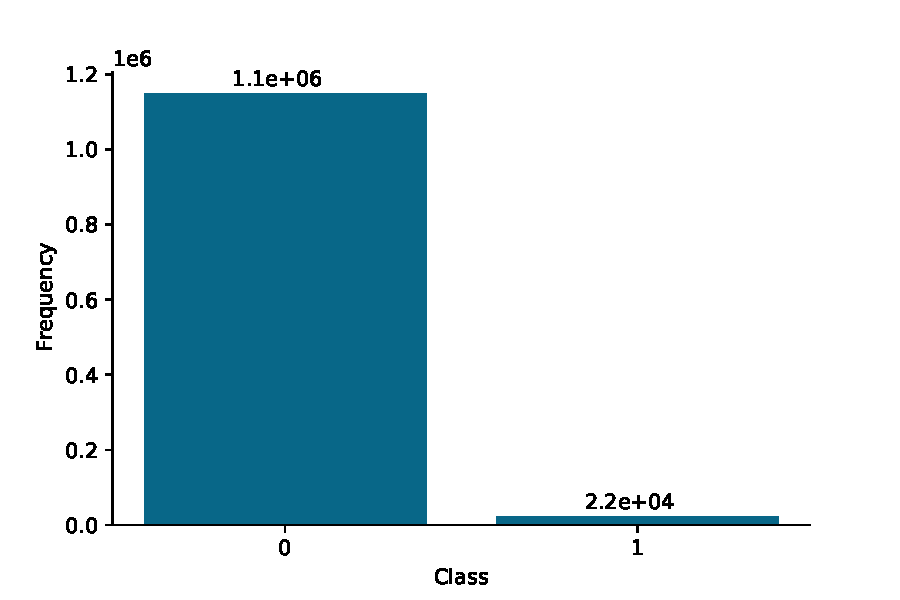
\includegraphics[scale = 0.7]{Label_dist.pdf}
    \caption{Breakdown of Target Variable}
    \label{fig:label_dist}
\end{figure}

\par The data used in Sindwani's model consist of vital signs, laboratory values, and demographic variables. We share some summary statistics in Table \ref{tab_describe}. The vital signs include data such as heart rate, pulse oximetry, temperature, and systolic blood pressure. These vital signs are collected on a regular basis and hence we can clearly see that they have fewer missing values. Laboratory values are the result of blood and other tests. These include variables such as fraction of inspired oxygen and glucose. Patients are less frequently tested and hence we can clearly see that these data are much more sparse than the vital signs data. The behavior of the missing is even clearer when looking at Figure \ref{fig:var_missings}. Figure \ref{fig:var_dists} provides the distributions of the continuous variables. We see that most variables are normally or log normally distributed. 

\begin{table}
\centering
\caption{Summary Statistics}
\label{tab_describe}
\begin{tabular}{lcccccc}
\toprule
{} &   Mean & Standard Deviation &  Minimum & Median & Maximum & Percent Missing \\
\midrule
Heart Rate (bpm)                 &  84.75 &              17.20 &    20.00 &  84.00 &  280.00 &            0.09 \\
Pulse oximetry (\%)               &  97.21 &               2.93 &    20.00 &  98.00 &  100.00 &            0.13 \\
Temperature (Celsius)            &  36.99 &               0.78 &    20.90 &  37.00 &   42.22 &            0.66 \\
Systolic blood pressure (mm Hg)  & 122.75 &              22.69 &    20.00 & 120.00 &  296.00 &            0.15 \\
Mean arterial pressure (mm Hg)   &  81.13 &              15.97 &    20.00 &  79.00 &  300.00 &            0.12 \\
Diastolic blood pressure (mm Hg) &  62.78 &              13.68 &    20.00 &  61.00 &  300.00 &            0.37 \\
Respiration Rate (bpm)           &  18.75 &               5.22 &     1.00 &  18.00 &  100.00 &            0.14 \\
Fraction of inspired oxygen (\%)  &   0.56 &              11.50 &     0.00 &   0.50 & 4000.00 &            0.90 \\
Serum glucose (mg/dL)            & 136.24 &              51.56 &    10.00 & 126.00 &  988.00 &            0.85 \\
ICU length-of-stay               &  27.07 &              28.69 &     1.00 &  21.00 &  336.00 &            0.00 \\
Type of ICU                      &   0.50 &               0.50 &     0.00 &   1.00 &    1.00 &            0.43 \\
Age                              &  62.34 &              16.29 &    14.00 &  64.24 &  100.00 &            0.00 \\
Gender                           &   0.57 &               0.50 &     0.00 &   1.00 &    1.00 &            0.00 \\
Hospital Admission Time          & -54.65 &             167.17 & -5366.86 &  -4.92 &   23.99 &            0.00 \\
\bottomrule
\end{tabular}
\end{table}


\begin{figure}[htbp!]
    \centering
    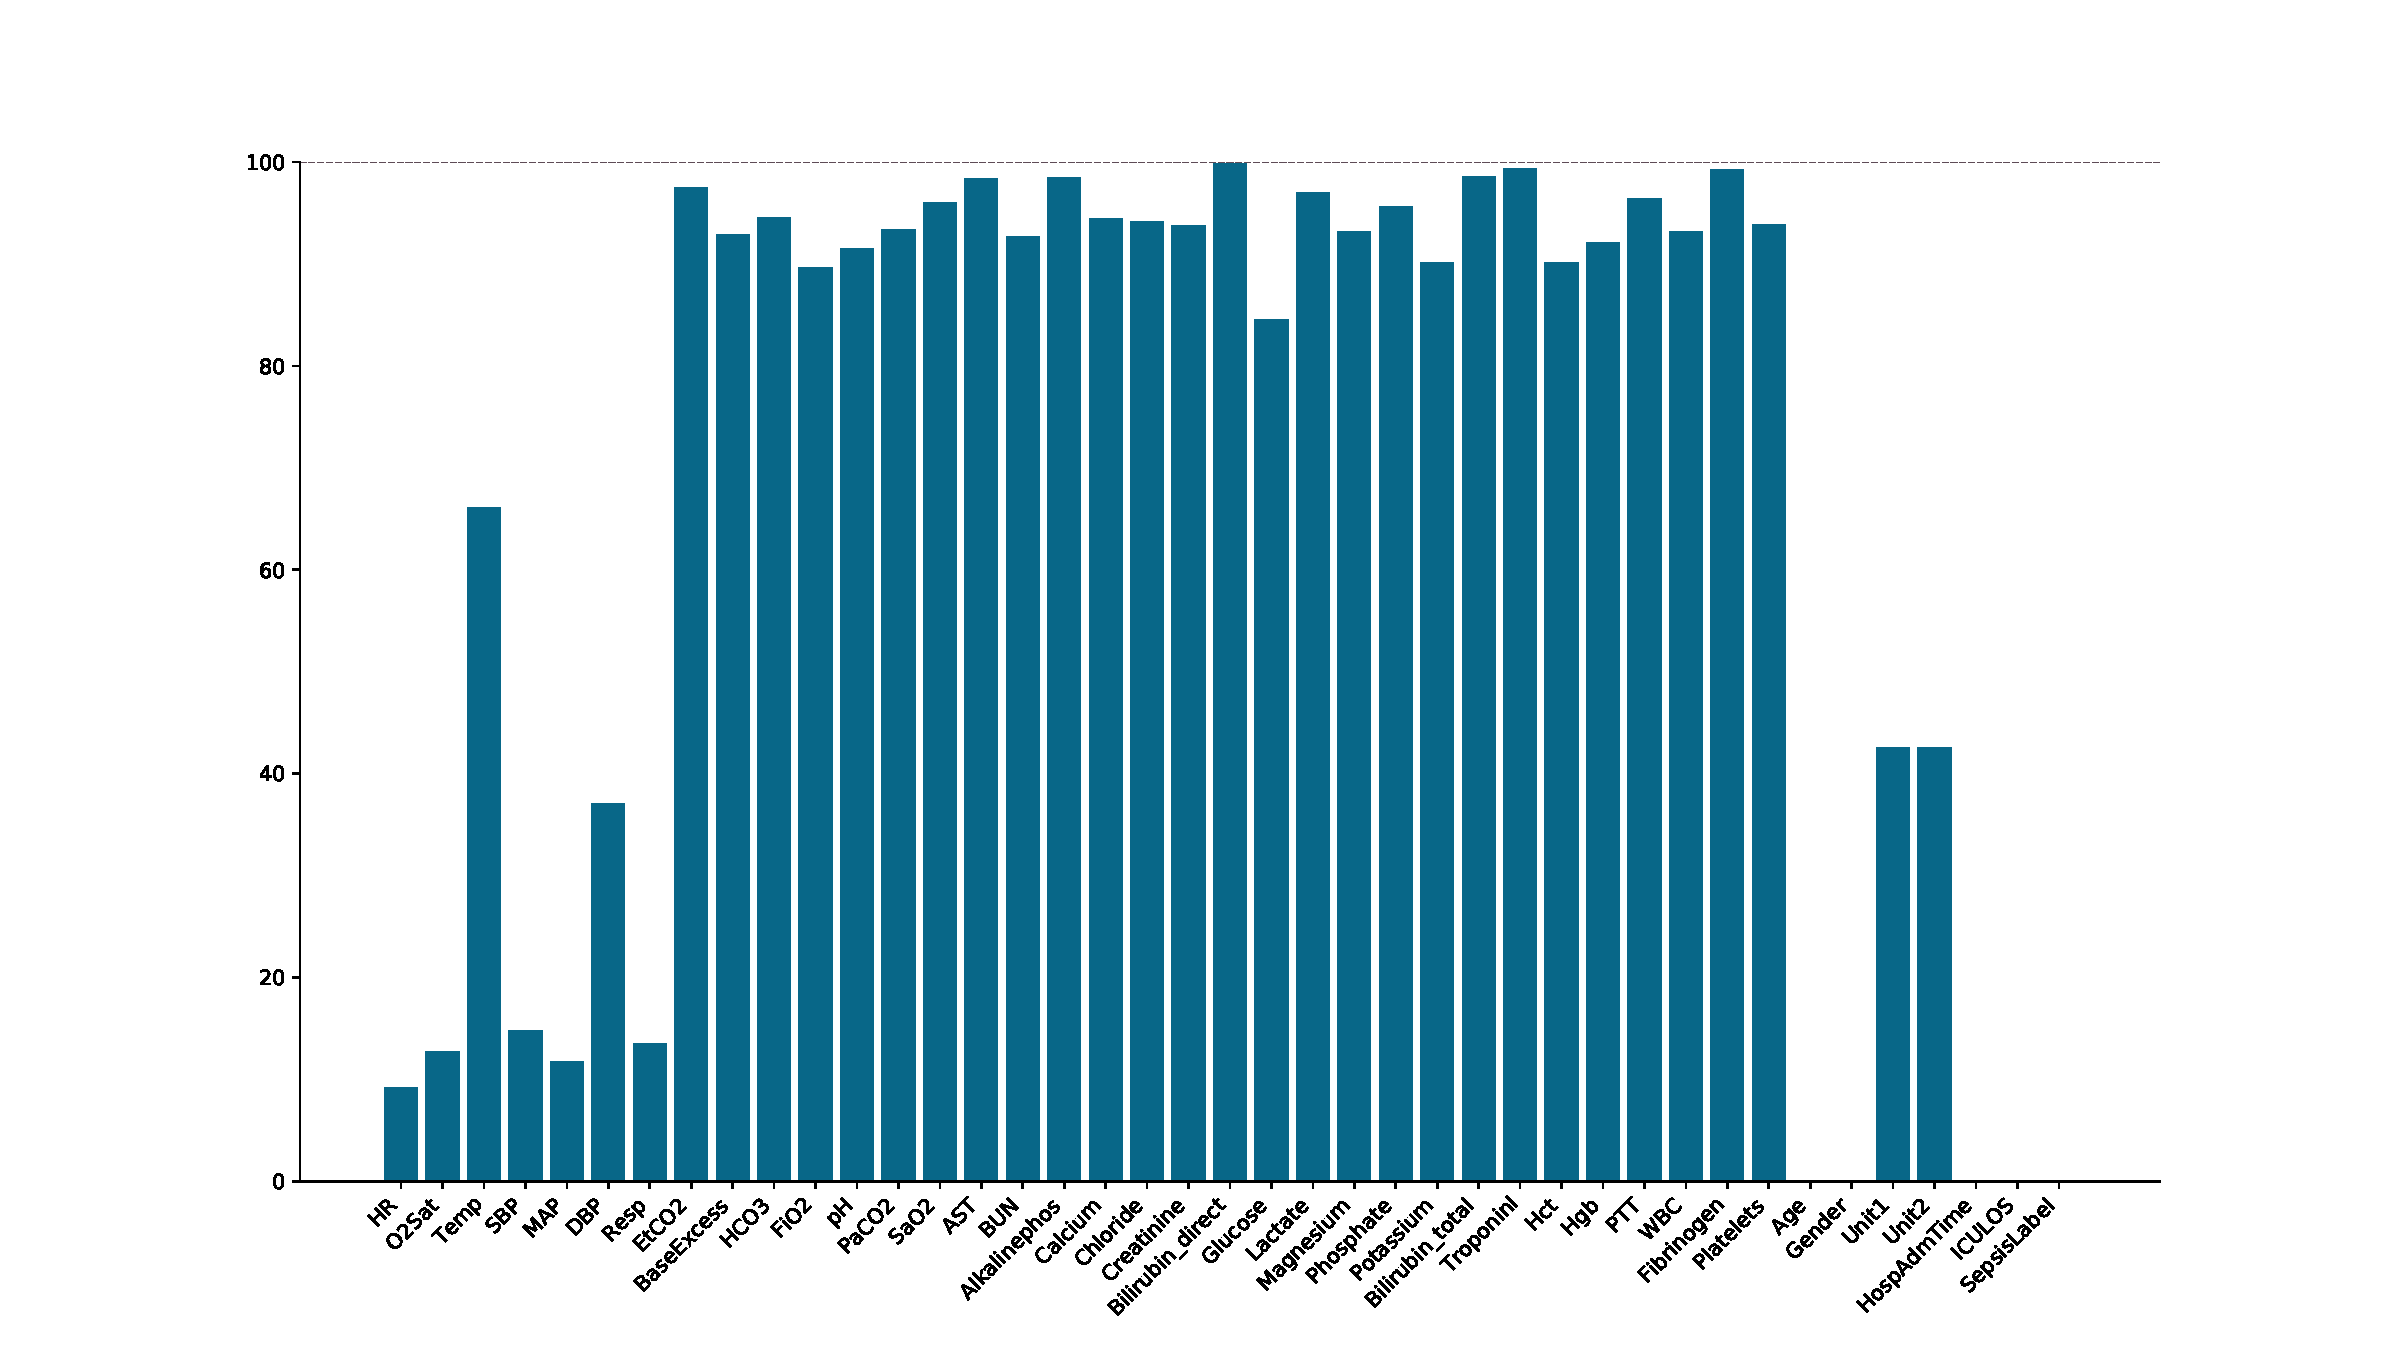
\includegraphics[scale = 0.45]{var_missing_hist.pdf}
    \caption{Percentage Missing per Variable}
    \label{fig:var_missings}
\end{figure}

\begin{figure}[htbp!]
    \centering
    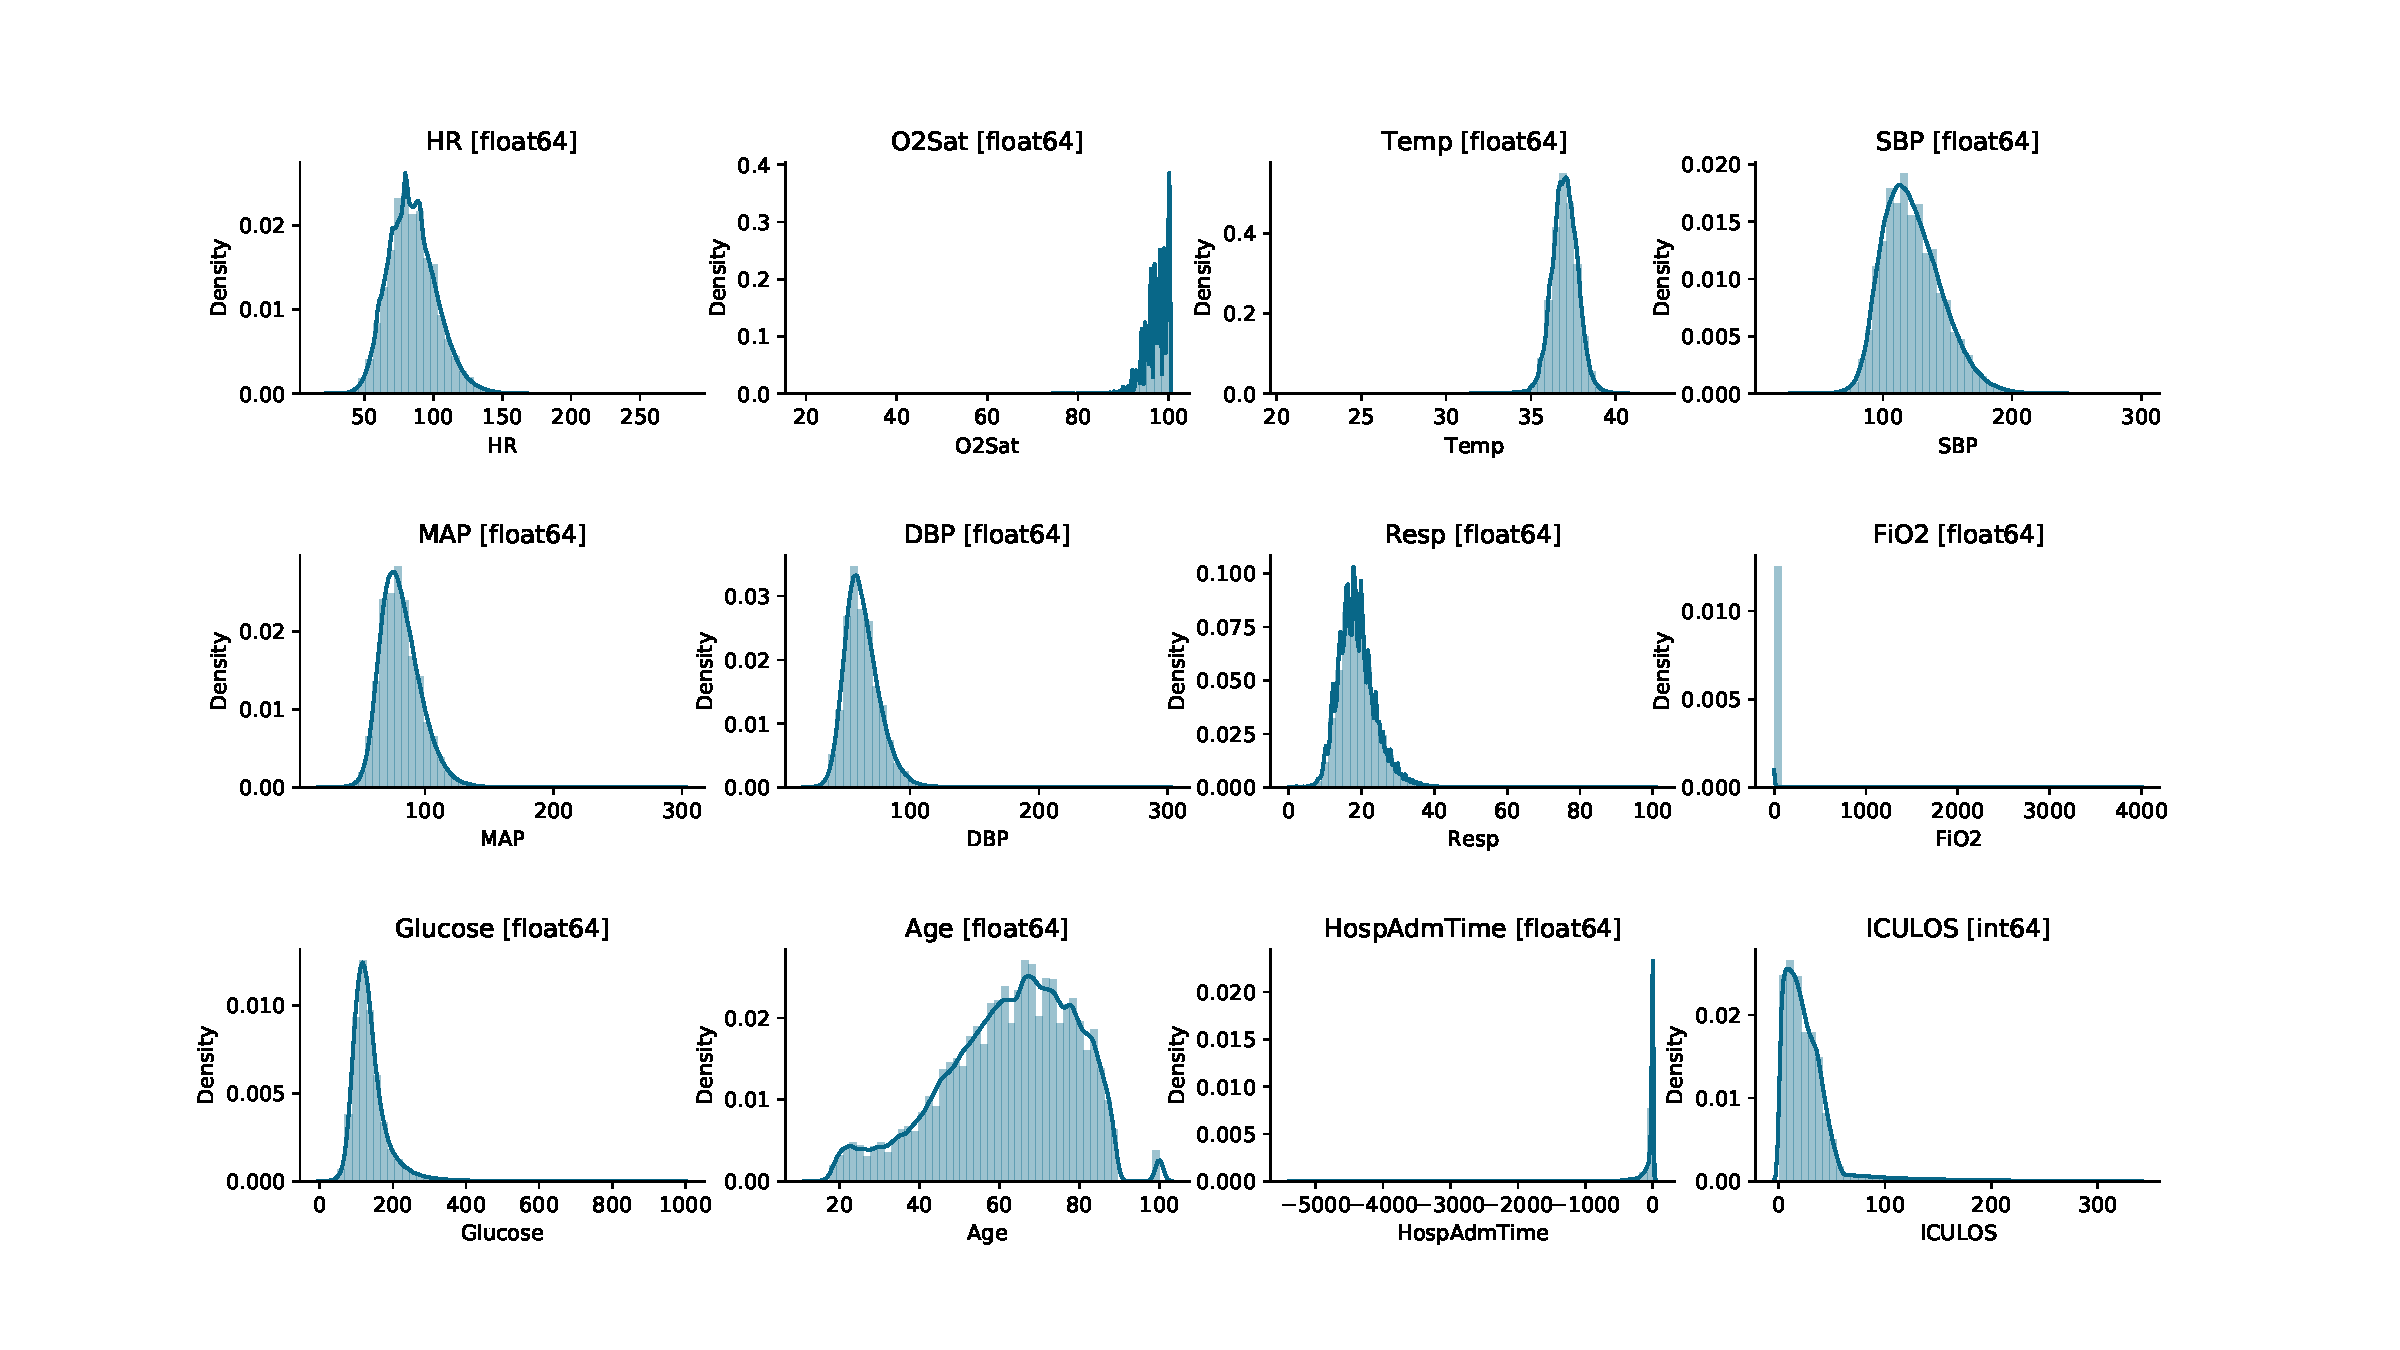
\includegraphics[scale = 0.45]{var_dists.pdf}
    \caption{Distributions of Continuous Variables}
    \label{fig:var_dists}
\end{figure}

\par An important aspect we need to look at is the breakdown of the sepsis label per category. Our data has two categories we take into account. One is the gender, which we will consider when evaluating fairness, and the other is the type of ICU (either surgical or medical). We can see the breakdown of the labels in figures \ref{fig:label_ICU} and \ref{fig:label_per_sex}. We can see that patients are 75\% and 12\% more likely to have sepsis in the medical ICU and as a male, respectively. It is also worth noting that we can see that for every woman in the data set there are 1.3 men. This means that men are over-represented in our sample.

\begin{figure}[hbtp!]
\centering
\begin{subfigure}[b]{0.45\textwidth}
    \centering
    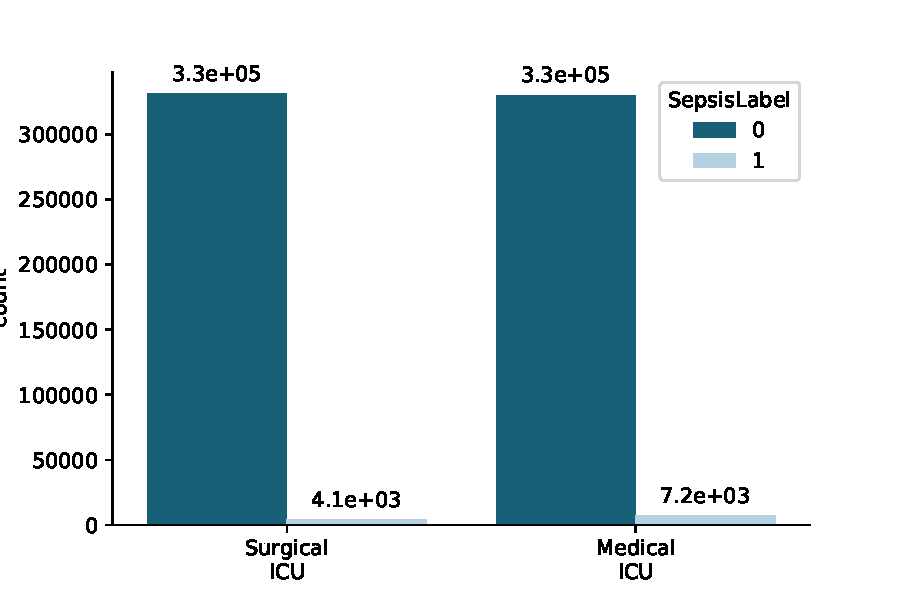
\includegraphics[scale = 0.6]{label_ICU.pdf}
    \caption{Type of ICU}
    \label{fig:label_ICU}
\end{subfigure}
\begin{subfigure}[b]{0.45\textwidth}
    \centering
    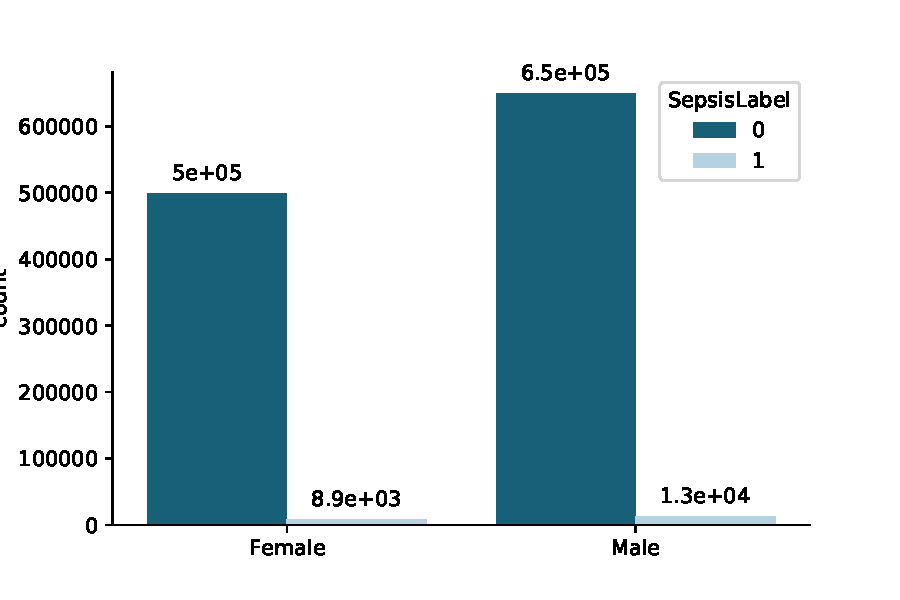
\includegraphics[scale = 0.6]{label_per_sex.pdf}
    \caption{Gender}
    \label{fig:label_per_sex}
\end{subfigure}
\caption{Sepsis by Categorical Variables}
\end{figure}

\par We see some interesting patterns in our the correlation heatmap, shown in Figure \ref{fig:corr_plot}. First, there is a strong correlation between the three measures of blood pressure included, and a strictly negative correlation between Unit1 and Unit2, which represent the medical and surgical ICU respectively. Interestingly, there is a high correlation between temperature and the medical ICU, and a high correlation between blood pressure and the surgical ICU. Another intuitively acceptable negative correlation is between the saturation of oxygen in the blood (O2Sat) and the respiratory rhythm (Resp). The more patients need to breath, the less oxygen is available in the blood. We also notice that older patients in general seem to have a lower blood pressure than a young patients. 

\begin{figure}[htpb!]
    \centering
    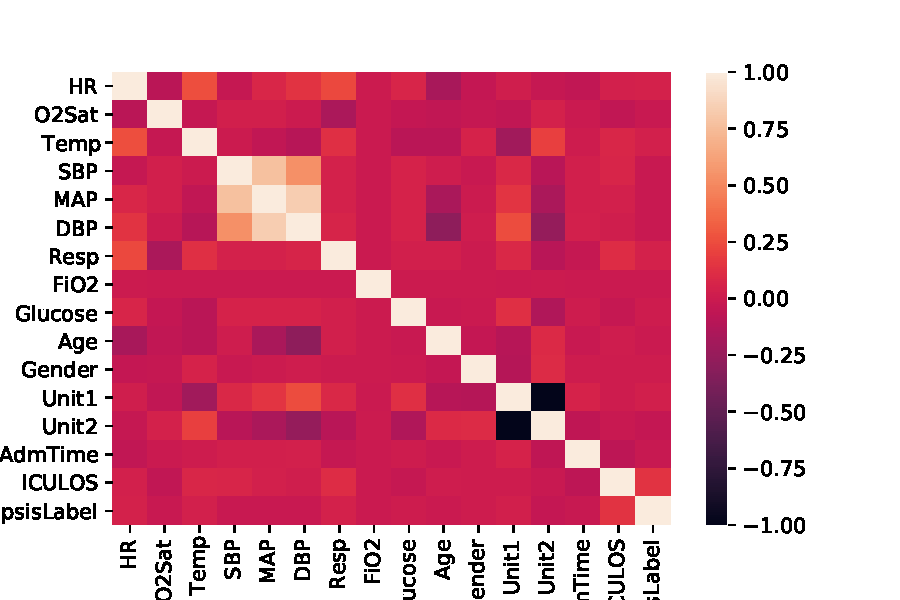
\includegraphics[scale = 0.7]{corr_plot.pdf}
    \caption{Correlation Plot}
    \label{fig:corr_plot}
\end{figure}

\section*{Implementation and validation}

% 3. Implementation and validation: present your understanding of the code that implements the ADS. This code was implemented by others (e.g., as part of the Kaggle competition), not by you as part of this assignment. Your goal here is to demonstrate that you understand the implementation at a high level.
%	a. Describe data cleaning and any other pre-processing
%	b. Give high-level information about the implementation of the system
%	c. How was the ADS validated? How do we know that it meets its stated goal(s)?

\par The main change made that has a serious impact on the composition of our data: the patient data was originally saved individually, but collected at different points in time. The designers of our model disregard this information and just use the data as if it were pulled from an identical distribution.

\par The authors of the model we will refer to made several data cleaning decisions. Instead of using the actual heart rates, they opted to categorize them in the categories normal, abnormal and missing. When determining the categories they took into account age but they did not take into account gender. This could potentially lead to a disparate impact down the road. They made similar changes for temperature, pulse oximetry and respiration rate. They also grouped individuals in categories based on age such as infant (< 1 year), child/adult (between 1 and 65 year old) and old (> 65 year). For the different blood pressures they distinguished between low, normal, elevated, high and missing.

\par The system is implemented as a prediction algorithm to predict sepsis within 6 hours of the input attributes. The system was validated by simple metrics, with little consideration for the impact of false positive and false negative rates. The authors have focused on recall, precision and average precision. Their best model was a decision tree which yielded:
\begin{itemize}
    \item Recall: 0.0978
    \item Precision: 0.0609
    \item Average Precision: 0.0195
\end{itemize}
In Table \ref{tab:conf_mat} we can see the confusion matrix of their final model. While overall accuracy (96.4\%) might have been good the recall rate is abysmal. Only a small fraction of those patients that will develop sepsis will be detected by this model. These are rates which would lead us to suggest not to use this model in practice. When optimizing the model, the designers were maximizing for the best possible recall and precision rates. This is in line with their goal of successfully catching positives. Nevertheless their goal does not take the disparate impact of the model on different subgroups into account. We will take a closer look at this in the next section.
\begin{table}[htpb!]
    \centering
    \begin{tabular}{l|cc}
        True\textbackslash{}Predicted & 0       & 1    \\ \hline
        0                             & 183 401 & 4330 \\
        1                             & 2591    & 281 
    \end{tabular}
    \caption{Confusion Matrix}
    \label{tab:conf_mat}
\end{table}

\section*{Outcomes}

% 4. Outcomes
%	a. Analyze the effectiveness (accuracy) of the ADS by comparing its performance across different subpopulations.
%	b. Select one or several fairness or diversity measures, justify your choice of these measures for the ADS in question, and quantify the fairness or diversity of this ADS.
%	c. Develop additional methods for analyzing ADS performance: think about stability, robustness, performance on difficult or otherwise important examples (in the style of LIME), or any other property that you believe is important to check for this ADS.

\par First, we will analyze the effectiveness of the ADS and verify that the results match those published by the author of the github using the same metrics as originally published. Then, we will run the ADS using the same metrics on only the male population and only the female population. We will then test additional fairness metrics to determine if the ADS system may result in bias. We would like to know if the metric produces disparate impact, and whether the mean difference is within an acceptable range. Given the implications highlighted in the introduction regarding the importance of false positives and false negatives in this context, we will also explore the false positive and negative rates across populations to evaluate the way in which the ADS makes mistakes and whether this may cause additional negative impact on the marginalized groups.

\clearpage

\section*{Summary}

% 5. Summary
%	a. Do you believe that the data was appropriate for this ADS?
%	b. Do you believe the implementation is robust, accurate, and fair? Discuss your choice of accuracy and fairness measures, and explain which stakeholders may find these measures appropriate.
%	c. Would you be comfortable deploying this ADS in the public sector, or in the industry? Why so or why not?
%	d. What improvements do you recommend to the data collection, processing, or analysis methodology?

\par We plan on first looking at the methodology and using disparate impact and difference in outcome to evaluate the possibly unfair impact of the model on the well-being of the patient from marginalized groups. At this point, we would not be comfortable using this system in healthcare settings, as ignoring the temporal nature of sepsis could have potentially disastrous effects on both men and women. One improvement we would suggest is taking into account how patients change over time and tweaking the model in such way that we are able to predict sepsis ex-post rather than identifying it as it occurs.

\newpage
\bibliographystyle{apacite}
\bibliography{references}
\end{document}